\chapter{Triangles in triangles (a proof without words)}
\label{cha:TrianglesInTriangles}
\begin{theorem}
There are $\binom{n+2}{4}$ equilateral triangles with vertices in a triangular
region of the triangular grid with $n$ vertices on each side.
\end{theorem}
\begin{proof}
The following is a bijection without words from a choice of four integers
satisfying \[
  1 \leq A < B < C < D \leq n + 2
\]
to equilateral triangles in the $n$-vertices-per-side triangular grid.
(Specifically, we have illustrated the case where
$n = 10$, $A = 4$, $B = 5$, $C=6$, and $D=10$.)

\noindent
\begin{center}
  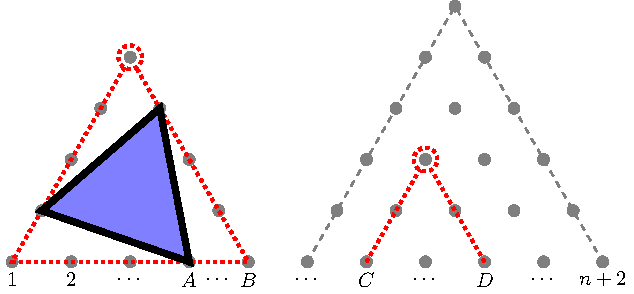
\includegraphics[scale=1]{figures/TrianglesInTriangles/assets/triangles_in_triangles_subset}
  \\
  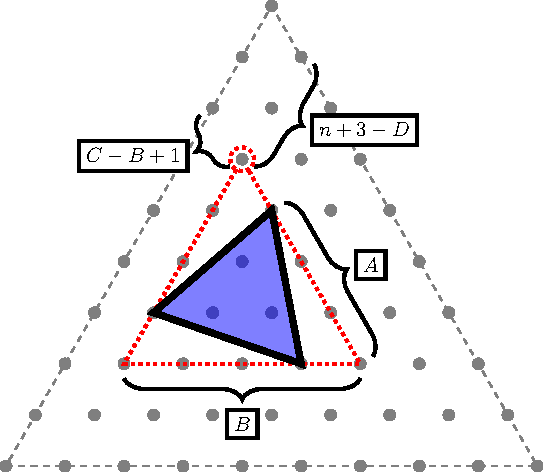
\includegraphics[scale=1]{figures/TrianglesInTriangles/assets/triangles_in_triangles}
\end{center}
\end{proof}
